\chapter{Lab Description}
\label{chp:lab_syllabus}

% \section*{Course Calendar Description}

% \subsection*{Math 112: Calculus I}
% An introductory course in differential calculus for science and engineering students, beginning with a review of basic algebra, equations and inequalities, analytic geometry, functions and graphs. Further topics include limits; continuity; rate of change; the derivative; differentiation of algebraic, trigonometric, exponential, logarithmic and inverse trigonometric functions; local and global extrema; Mean Value theorem; graph-sketching; related rates; linear approximation; L’Hopital’s Rule; optimization; Newton’s method. 

% \subsection*{Math 122: Calculus II}
% This course is a continuation of MATH 112. Topics include antiderivatives; the definite integral; Fundamental Theorem of Calculus; applications of integration including area, volume, average value; techniques of integration; numerical integration; improper integrals; introduction to differential equations; direction fields; Euler’s method; separable differential equations and applications; infinite sequences and series; convergence; power series; Taylor series and Taylor polynomial approximation.

\section*{Purpose of Lab}
Your lab section is designed to supplement the content that you are learning in lecture. You will be applying those lecture topics during the lab through Maple, which is a powerful computational software. It is the goal of the lab to aid in your understanding of calculus as well as introduce you to the tools of mathematics that are available through computers.

\section*{Lab Expectations}
Each week you will work on a new activity from this lab manual. Your lab instructor will inform you of which activity you will be working on each week. You must complete each component of each activity individually. Plagiarism of lab work will not be tolerated.

\begin{marginfigure}
    \centering
    \begin{tikzpicture}[auto]
    	% place nodes
    	\node [rectangle, draw, text centered, rounded corners, text width=10em] (read) {Read through activity and tutorials};
    	\node [ellipse, draw, text centered, rounded corners, text width=10em, below=1cm of read] (readquiz) {Complete reading quiz};
    	\node [rectangle, draw, text centered, rounded corners, text width=10em, below=1cm of readquiz] (activity) {Complete exercises from lab manual in Maple};
    	\node [rectangle, draw, text centered, rounded corners, text width=10em, below=1cm of activity] (save) {Save file(s)};
    	\node [ellipse, draw, text centered, rounded corners, text width=10em, below=1cm of save] (quiz) {Complete activity quiz and submit file(s)};
    	% Draw edges
    	\path [draw, -latex'] (read) -- (readquiz);
    	\path [draw, -latex'] (readquiz) -- (activity);
    	\path [draw, -latex'] (activity) -- (save);
    	\path [draw, -latex'] (save) -- (quiz);
    \end{tikzpicture}
    \caption{Workflow for each weekly activity.}
\end{marginfigure}

\subsection*{Prior to lab} 
Before lab, read through the activity as well as the recommended tutorials from the back of the book. Once you have read through the instructions and tutorials, you will need to complete the \textbf{reading quiz} for the activity.

\marginnote[1cm]{Some lab computers take a couple minutes to log into. Always give yourself a few extra minutes at the start of lab to log in.}

\subsection*{Start of lab}
After logging into the school computer, you should begin by opening up the latest version of Maple as well your lab section's Moodle page. You are expected to have this lab manual with you during lab and you should complete all exercises in order. It is a great idea to have a pen or pencil handy to take notes in your manual while you complete the exercises. Your lab instructor will be available to assist you with the activity, though you will find that many of your questions can be answered by looking through the tutorial sections at the back of this book.

\marginnote[-.4cm]{Always bring your lab manual along to your lab. Take lots of notes in it!}

\subsection*{End of lab}
Once you have completed the exercises, make sure to save your work! You are now ready to complete the \textbf{activity quiz}. The questions in this quiz should be relatively quick to answer once you have completed the exercises from the activity. Often, you can simply copy and paste the output from Maple into the blanks on the quiz. You will be required to \textbf{submit your Maple work} in addition to the quiz.

\marginnote{The questions on your Moodle quiz relate to the exercises in this book. Make sure to finish your exercises prior to the quiz.}

\subsection*{Final lab}
During your final lab, you will be expected to complete an open-book \textbf{lab test}. The test will be based upon the activities that you have completed throughout the semester. You are permitted to have this manual during the test.

% \clearpage

% \section*{Evaluation}
% Your lab grade is determined as follows:
% %\begin{tcolorbox}
% \begin{table}[h]
% \centering
% \begin{tabular}{ll}
% Reading Quizzes                 & 15\%\\
% Activity Submission and Quizzes	& 60\%\\
% Lab Test		            	& 25\%\\
% \hline
% Total			            	& 100\%
% \end{tabular}
% \end{table}
% %\end{tcolorbox}
% \par Your lab grade is transferred to instructor of your lecture session at the end of the semester and accounts for 10\% of your overall Math 112/122 grade.

\section*{Lab Test}
During your lab test, you will be permitted the following materials:
\vspace*{-1ex}
\begin{multicols}{2}
\begin{itemize}
\item This lab manual
\item Handwritten notes
\item Maple help
\columnbreak
\item Previously completed activities
\vfill\null
\end{itemize}
\end{multicols}
\noindent The following are not allowed:
\vspace*{-1ex}
\begin{multicols}{2}
\begin{itemize}
\item Discussion with other students
\item Cell phones
\item Other electronic devices
\item Email
\item Internet (other than Moodle for file submission)
\vfill\null
\end{itemize}
\end{multicols}
You will be allowed to ask for clarification on questions, but will not be allowed to ask for assistance in completing a question or resolving an error in your work.
\par
You will be expected to submit your work electronically and any duplicate submissions will receive a grade of zero. It is important to save your work frequently in case your computer encounters a serious error.
\marginnote[-1cm]{Don't forget to save your file in your \textbf{network folder}. This folder is accessible from any computer. Saving your files is explained in detail in the next chapter.}

\chapter{Introduction to Maple}
\label{chp:introduction}

\section*{The Maple Computer Algebra System}
In lab, you will be using the latest version of Maple, which is a symbolic and numeric computing environment. Maple provides an interface for analyzing, exploring, visualizing, and solving mathematical problems. The interface also allows you to maintain an easy-to-follow document so that you can retrace your thought process. If you plan to pursue any branch of mathematics or field that relies on mathematics, having basic knowledge of a computer algebra system is a very useful tool.

\section*{How to Use This Manual}
This book is divided into two main parts:
\begin{itemize}
\item[\textbf{Part \ref{pt:Activities}}] consists of activities for you to complete. These activities are divided into two chapters: Math 112 and Math 122. Each activity focuses on one topic from that course and contains a list of exercises for you to complete with Maple. Some of these exercises may give very explicit instructions for typing a command into Maple, while others may require you to use your own intuition and understanding of the capabilities of Maple.
\item[\textbf{Part \ref{pt:Tutorials}}] consists of several chapters that provide examples of the usage of common commands in Maple. Many of these examples are designed to be minimalistic in order to show you their basic usage. Each of these examples was completed within Maple and should be reproducible on your own computer.
\end{itemize}
At the beginning of each activity, a list of the most relevant tutorials is given. It is expected that you read through those tutorials as you complete the exercises of that activity. Many activities build upon previously learned commands, so it is a good idea to thoroughly read through all of the relevant tutorials as you progress through lab.

\section*{Accessing Maple and Saving Your Work}
Maple is installed on all lab computers as well as on computers in the library. However, personal copies of Maple are not available through Okanagan College at this time.

\subsection*{Opening Maple on School Computers}

\begin{marginfigure}
\centering

\includegraphics[width=1cm]{introduction/figures/horizonvmware.png}
\caption{You may need to open the VMware Horizon Client first using this desktop icon.}
\end{marginfigure}

On some Windows computers, the most recent version of Maple may be installed directly. In this case, you can simply hit the Start Menu key on your keyboard (in the lower left corner) and begin typing the word "Maple". If Maple is installed directly, then Windows Search will automatically find the version installed and display a link to the application. Alternatively, you should be able to find Maple by browsing the list of installed programs on the Start Menu.

On other computers, you may need to log into a virtual machine to access Maple remotely. On these machines, you will typically find a link to VMware Horizon Client on the desktop. You will need to open this client and log into the remote machine using the same information as you previously used to log into the computer. Once the remote machine loads, you should find Maple in the Start Menu as described above.

\begin{marginfigure}[-5cm]
\centering
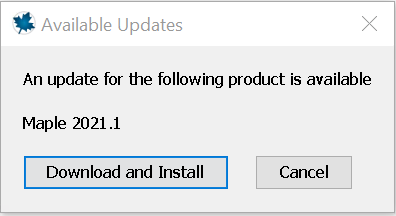
\includegraphics[width=5cm]{introduction/figures/mapleupdate.png}
\caption{After opening Maple, you may be prompted to update the version. You can click Cancel on this dialog box.}
\end{marginfigure}

\subsection*{Organizing Files in your Network Folder}

\begin{marginfigure}
\centering

\includegraphics[width=1.5cm]{introduction/figures/networkfoldershortcut.png}

\includegraphics[width=1cm]{introduction/figures/fileexplorer.png}
\caption{The shortcut for your network folder is on the desktop. You can also open File Explorer with the shortcut on the taskbar.}
\end{marginfigure}

You are given your own personal folder on the network in which to save your files. This folder is accessible from any computer on campus and from VMware Horizon, so you should save all of your work in this folder. You can find this folder by using the desktop shortcut or by opening up File Explorer and clicking on This PC.

\begin{figure}
\centering
\adjincludegraphics[width=0.9\textwidth,trim={0 {0.3\height} 0 0},clip]{introduction/figures/thispc}
\caption{Your network folder should appear under This PC when using File Explorer.}
\end{figure}

\clearpage

It is best to create a new subfolder in your network folder for your lab. This folder could be called something like "Math 112 Labs" so that it is easy to find and organize all of your saved Maple files. When you wish to save your file in Maple, now you can navigate to this folder and save your file with the name of the activity.

\begin{figure}
\centering
\adjincludegraphics[width=0.9\textwidth,trim={0 {0.3\height} 0 0},clip]{introduction/figures/fileorganization}
\caption{Make sure to create a folder for your lab inside your network folder. Save all of your files here using obvious names so that they are easy to find again later.}
\end{figure}

The files that Maple saves are only readable through Maple. However, you can find the Export As tool under the File menu. From there, you can change the file type to PDF and save your document. PDF files can be read by other programs, but cannot be edited by Maple.

\begin{figure}
\centering
\adjincludegraphics[width=0.3\textwidth,trim={0 {0.3\height} {0.2\width} 0},clip]{introduction/figures/exportas}
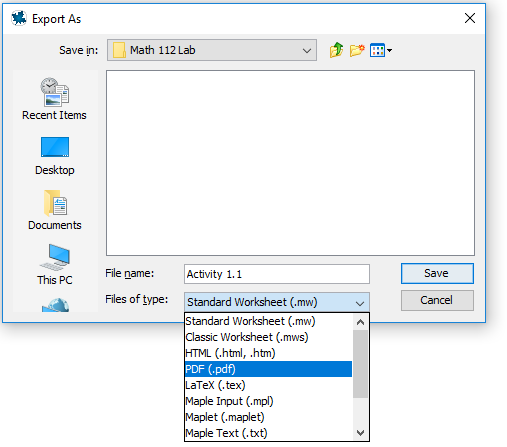
\includegraphics[width=0.6\textwidth]{introduction/figures/exportpdf.png}
\caption{You can export your Maple worksheet as a PDF file type, which can be opened on most devices without Maple. However, Maple cannot edit PDF files.}
\end{figure}

The files that you have saved on your network folder on campus can be accessed from home through a browser by using the following address:

\begin{center}
    \url{https://myfiles.okanagan.bc.ca/}
\end{center}